\documentclass{ximera}

\author{Bart Snapp}

\title{About Ximera}


\begin{document}


Ximera, pronounced ``chimera,'' (\textbf{X}imera:
\textbf{I}nteractive, \textbf{M}athematics, \textbf{E}ducation,
\textbf{R}esources, for \textbf{A}ll) is an open-source platform that
provides tools for authoring and publishing (PDF and Online),
open-source, interactive educational content, such as
textbooks, assessments, and online courses.  
\textbf{The ultimate goal of this project is to promote sustained student success and savings.}





\section*{Instructor Experience}


Instructors (who are not authors) can freely use any Ximera materials,
simply by using the the URL of the course. Moreover, if an instructor
experiences issues with the content or performance of the materials,
there are simple ways to report these issues. Since Ximera is built
using GitHub, see Section~\ref{ss:gh}, we use GitHub's issue tracking
feature. Moreover, since the content is open, and it is written in
\LaTeX, see Section~\ref{ss:LaTeX}, a language the instructors prefer
to use, instructors can actually submit fixes for the materials
themselves on GitHub. As an example, we've had 120 issues identified
and fixed by instructors in OSU's calculus series.




\section*{Author Experience}


 
With Ximera, authors use a document preparation system called
\LaTeX\ to create their content, see Section~\ref{ss:LaTeX}.  While
this system may seem obscure to the lay-person, it is in fact
enormously popular in mathematics and other STEM fields (on the
preprint arXiv, there are over 2 million papers, nearly all of which
were authored in \LaTeX). Most potential authors already have
materials written in \LaTeX. Due to the popularity of \LaTeX, it is a
natural authoring environment for writing STEM content.
\LaTeX\ allows authors to simultaneously produce PDFs and online
interactive content, see Figure~\ref{F:sout}.



 \begin{figure}
  \centering
  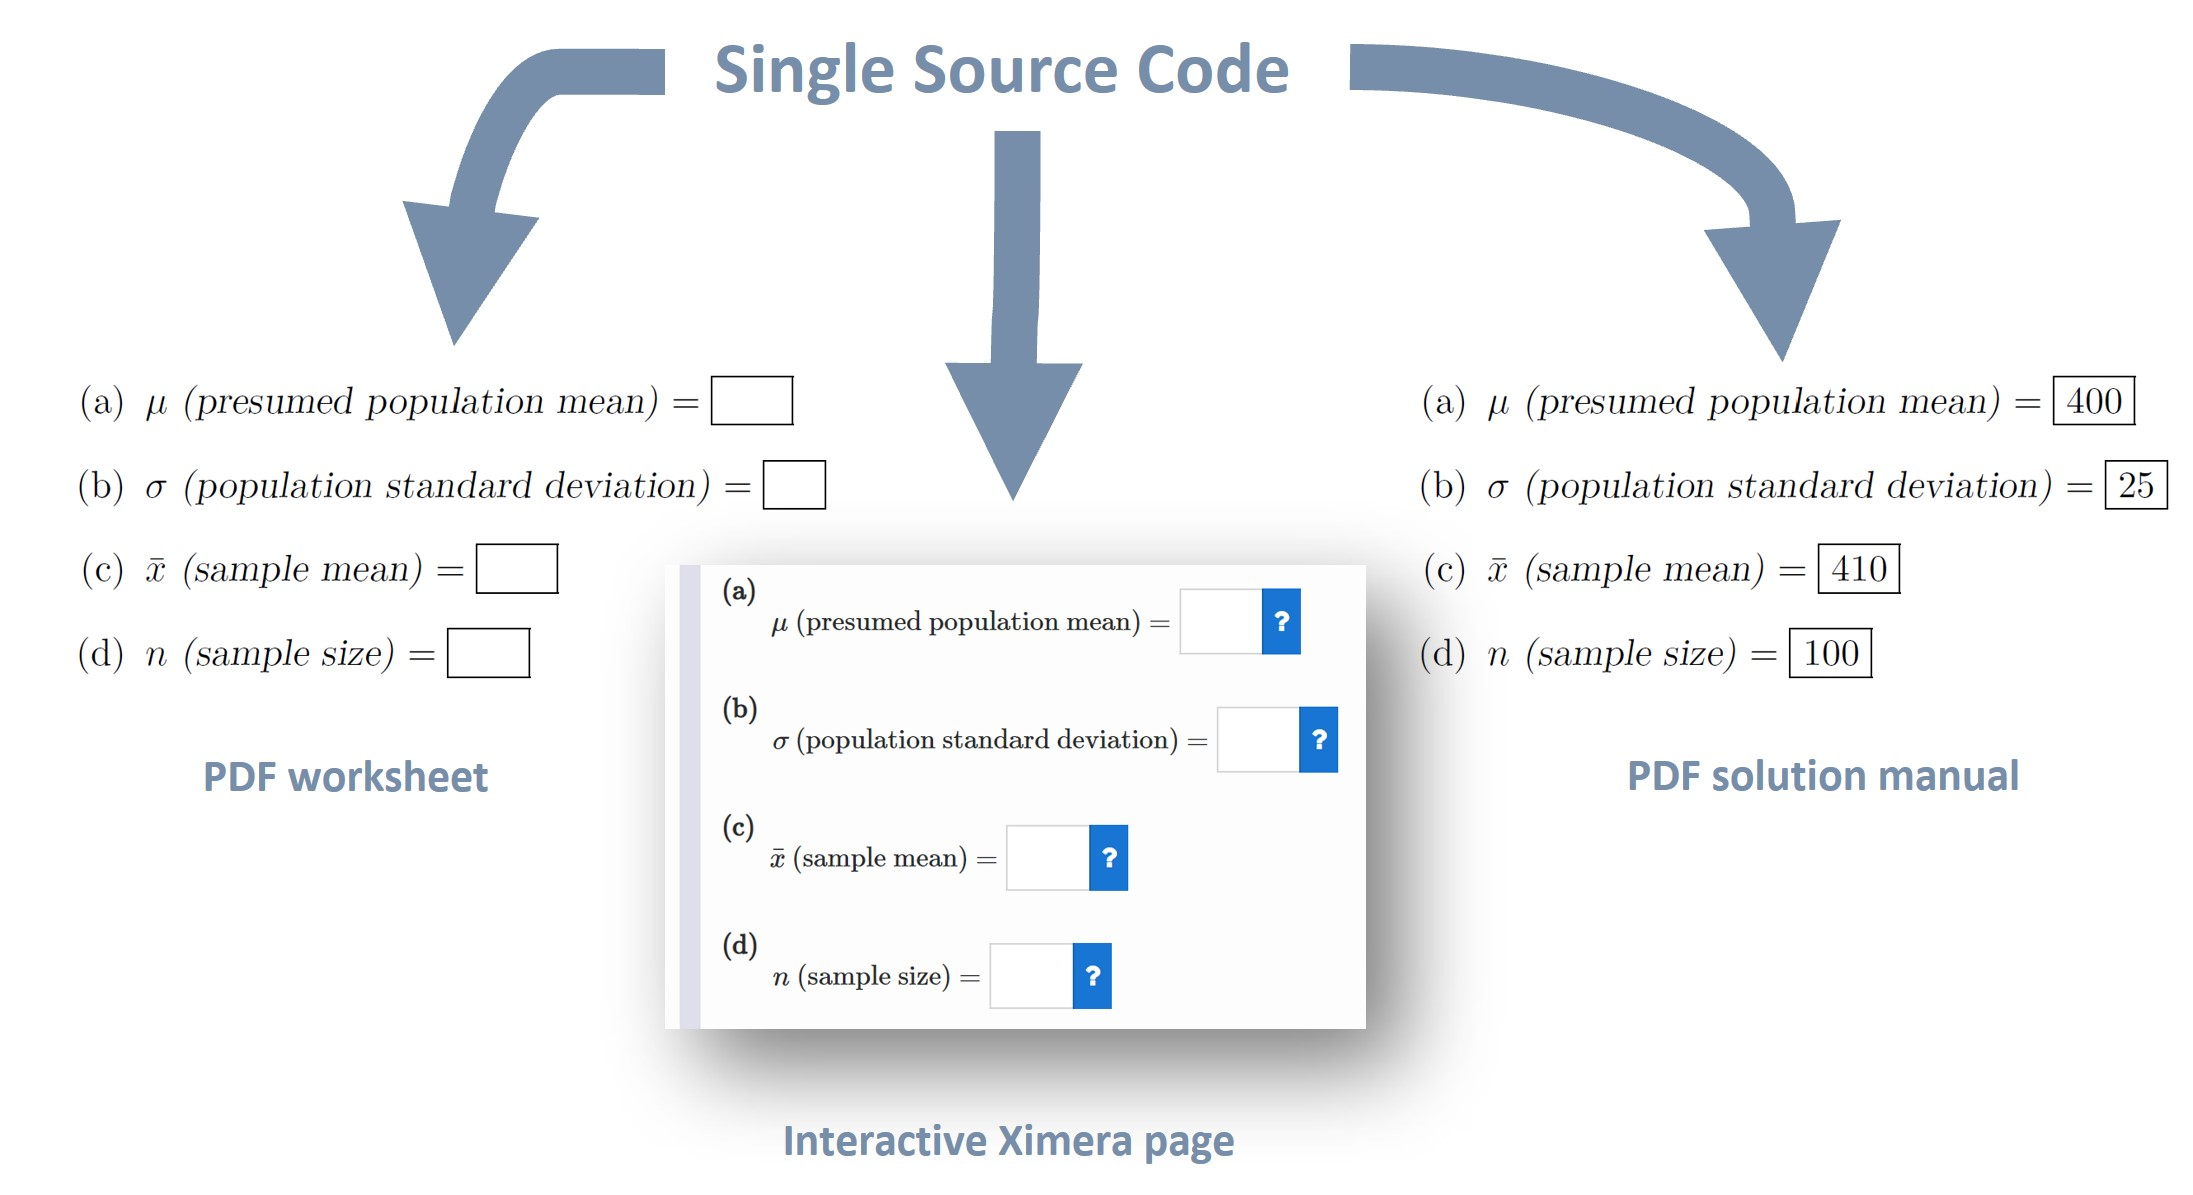
\includegraphics[width=.8\textwidth]{SimultaneousOutput.jpg}
  \caption{Single source code generates three different outputs.}
  \label{F:sout}
\end{figure}





\section*{Exceptional Design Elements in Ximera}


Ximera is built by educators, for educators. With this in mind, we'd
like to highlight three design elements of our project that we find
particularly powerful.


 \subsection*{Simultaneous Output}

 The Ximera platform provides an innovative approach by allowing
 authors to generate both PDF and interactive versions of their
 materials simultaneously. This approach enhances the accessibility
 and usability of the materials. The same Ximera materials can be used
 many different ways in a classroom, and this is very useful for
 authors and instructors.  Moreover, it allows students to access the
 content in the format that suits their learning preferences best.
 Finally, having a PDF version of the content provides a backup
 solution for students and instructors in case of technological
 difficulties during the learning process.


 


\subsection*{Open Community}

All the files used to make Ximera documents are licensed with
open license, with the content licensed under CC-BY-NC-SA.  All files
are hosted on GitHub, a web-based platform for version control and
collaborative software development.  This allows users to host and
review code, manage projects, and collaborate with others. As
discussed below, Ximera has grown a solid open source community on
GitHub. By hosting all content publicly on GitHub, Ximera allows for
transparent and collaborative development of educational materials,
which can be modified and adapted to meet the specific needs of
different learners and contexts.





All content is openly visible to anyone through an internet
search. The Ximera server is publicly accessible and does not require
users to log in to view the content. The Ximera project is committed
to open education and the democratization of knowledge. The project
aims to make educational materials freely and easily accessible to
anyone, anywhere, at any time.



These design elements promote equity and inclusivity in education by
providing access to high-quality materials to learners from diverse
backgrounds.




\subsection*{Immediate Feedback} 

The Ximera platform provides immediate feedback to students as they
work through the interactive content, enhancing their learning
experience and promoting student engagement. By using a client-side
computer algebra system, Ximera's interactive content gives students
instant feedback on the correctness of their answers, allowing them to
correct mistakes and reinforcing their learning. Additionally, the
answer-box feature of Ximera provides real-time feedback to students
as they work through problems, helping them to understand and correct
their mistakes as they go.

\end{document}
